\documentclass{article}
\usepackage[utf8]{inputenc}
\usepackage[total={8in,10in}]{geometry}
\usepackage{graphicx}
\graphicspath{{../plots/}}
\usepackage[font=Large,labelfont=bf]{caption}
\captionsetup{width=\linewidth}

\begin{document}
	
	\begin{figure}
			\centering 
			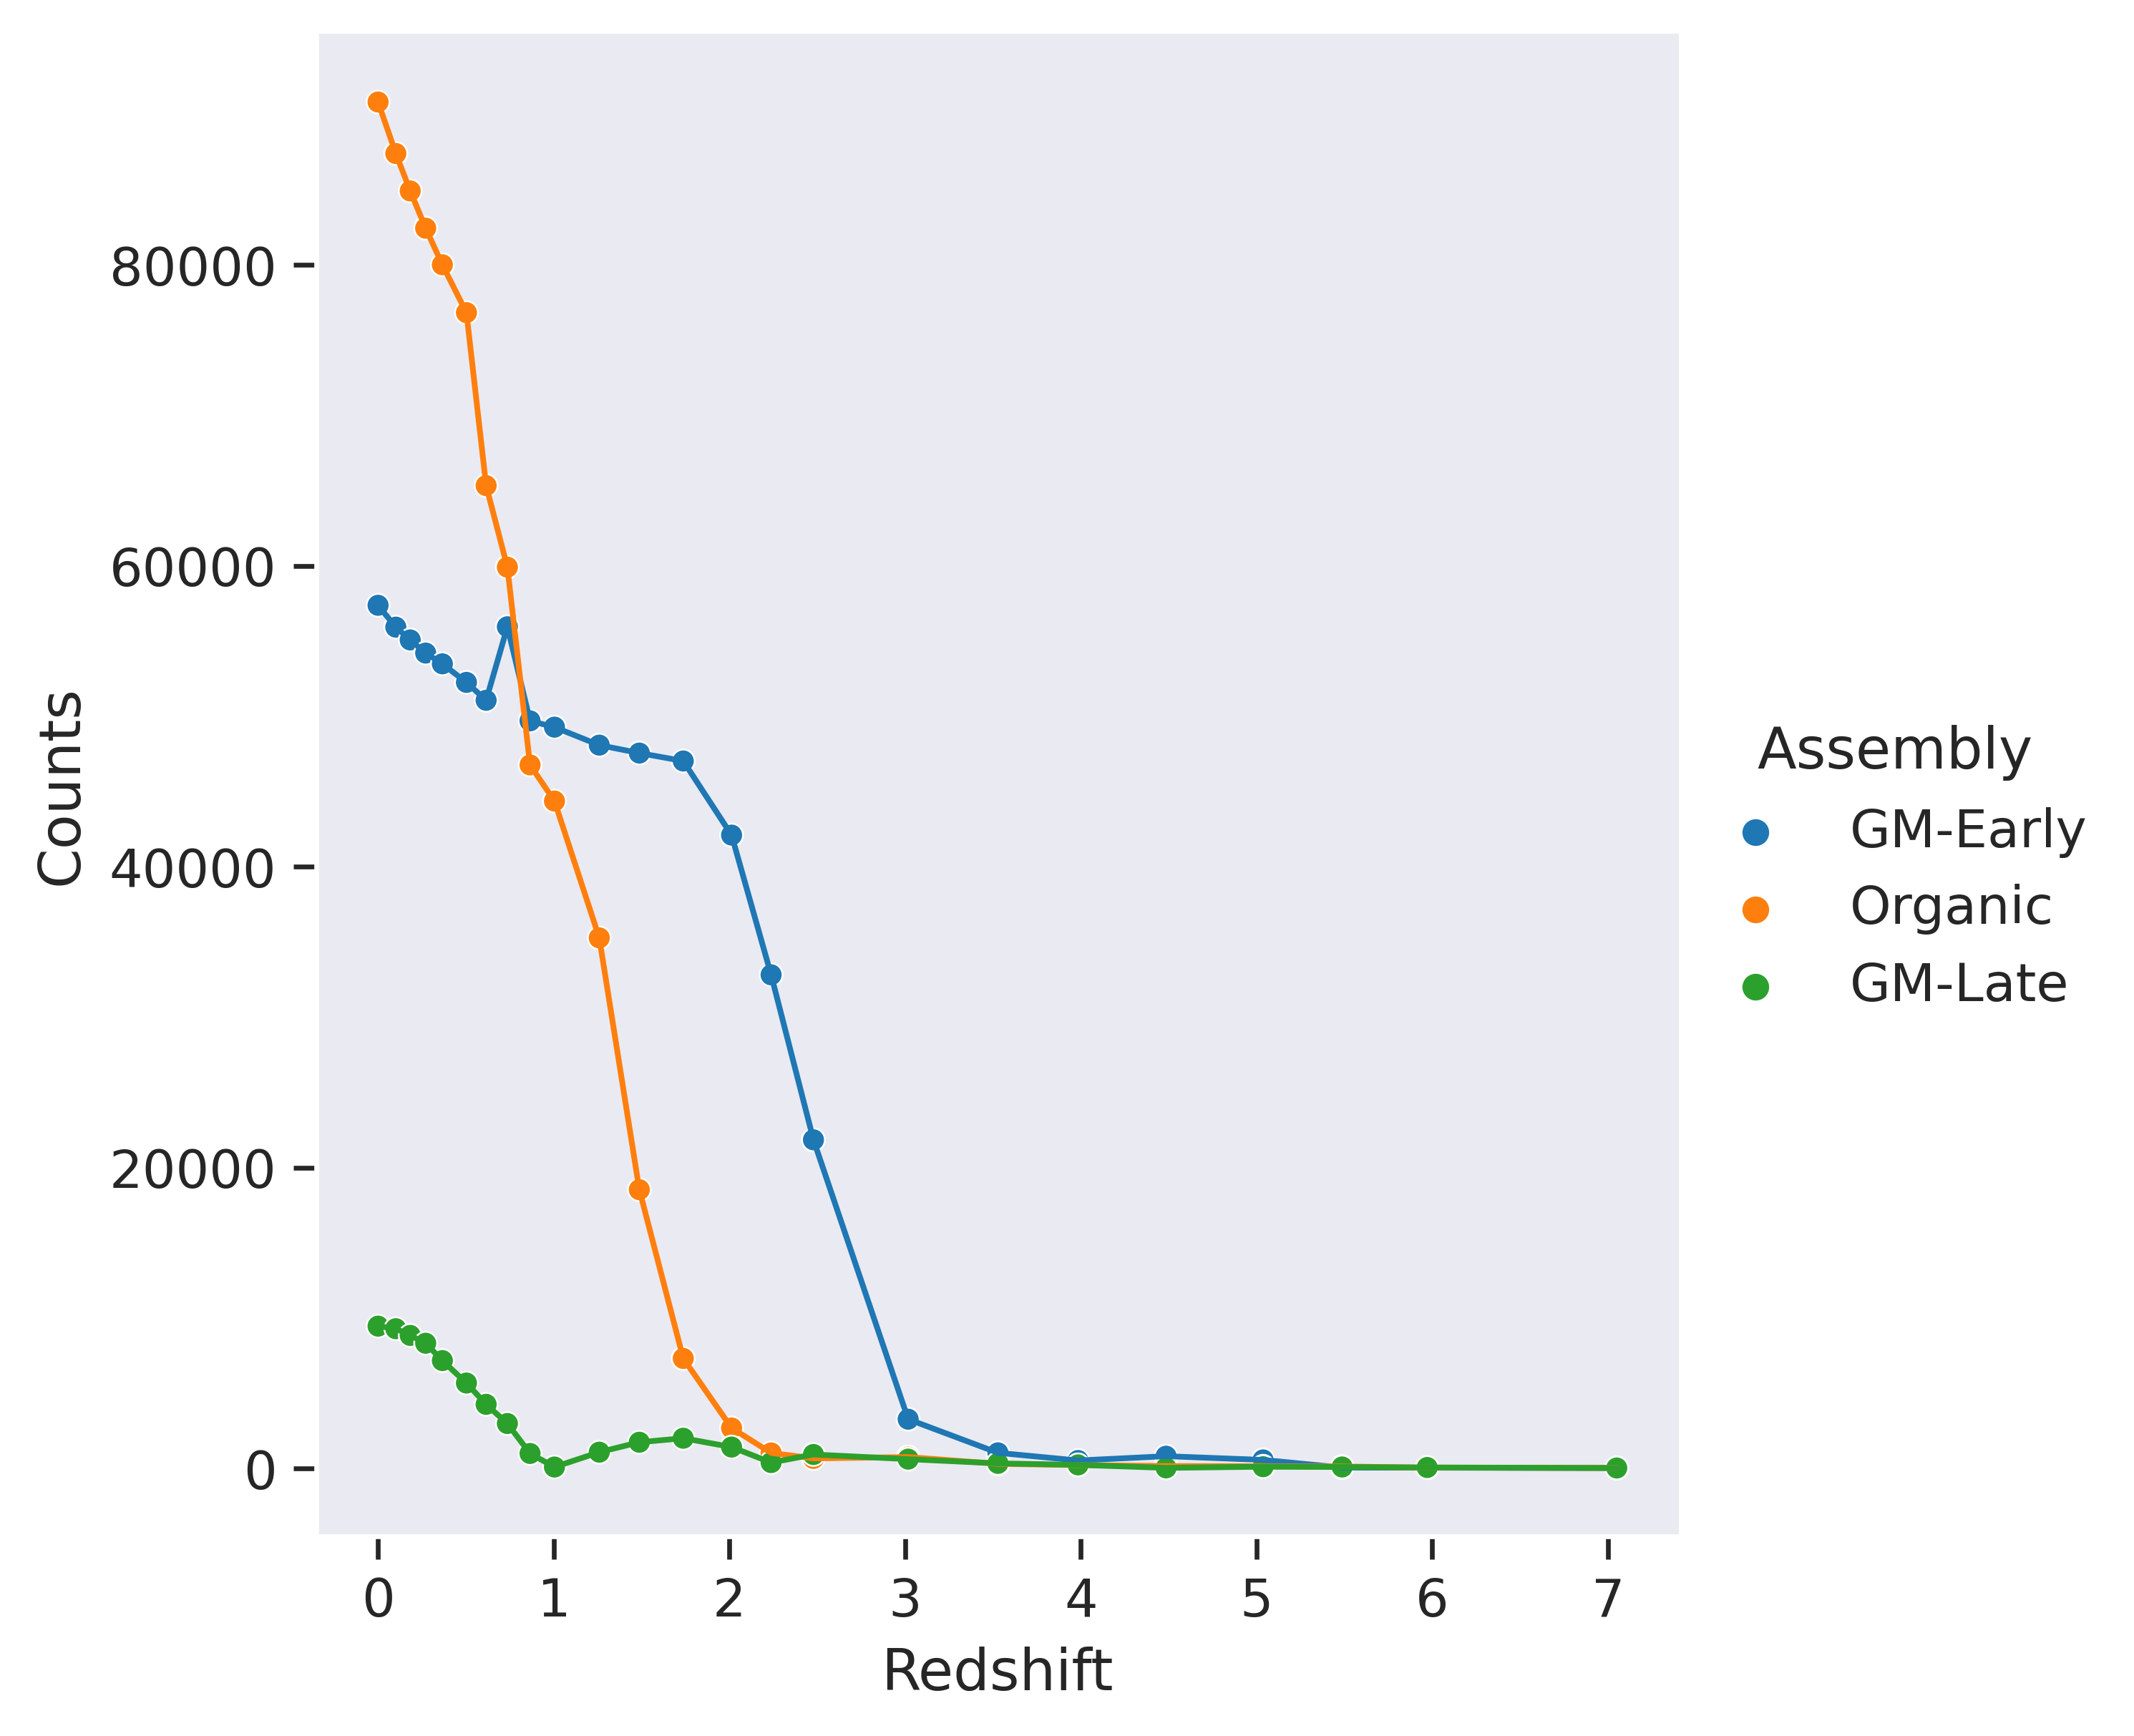
\includegraphics[width=.5\columnwidth]{../plots/particle_distribution_wrt_redshift.png}
			\caption{Distribution of particles with redshift for three assembly modes.}
	\end{figure}

	\begin{figure}
			\centering 
			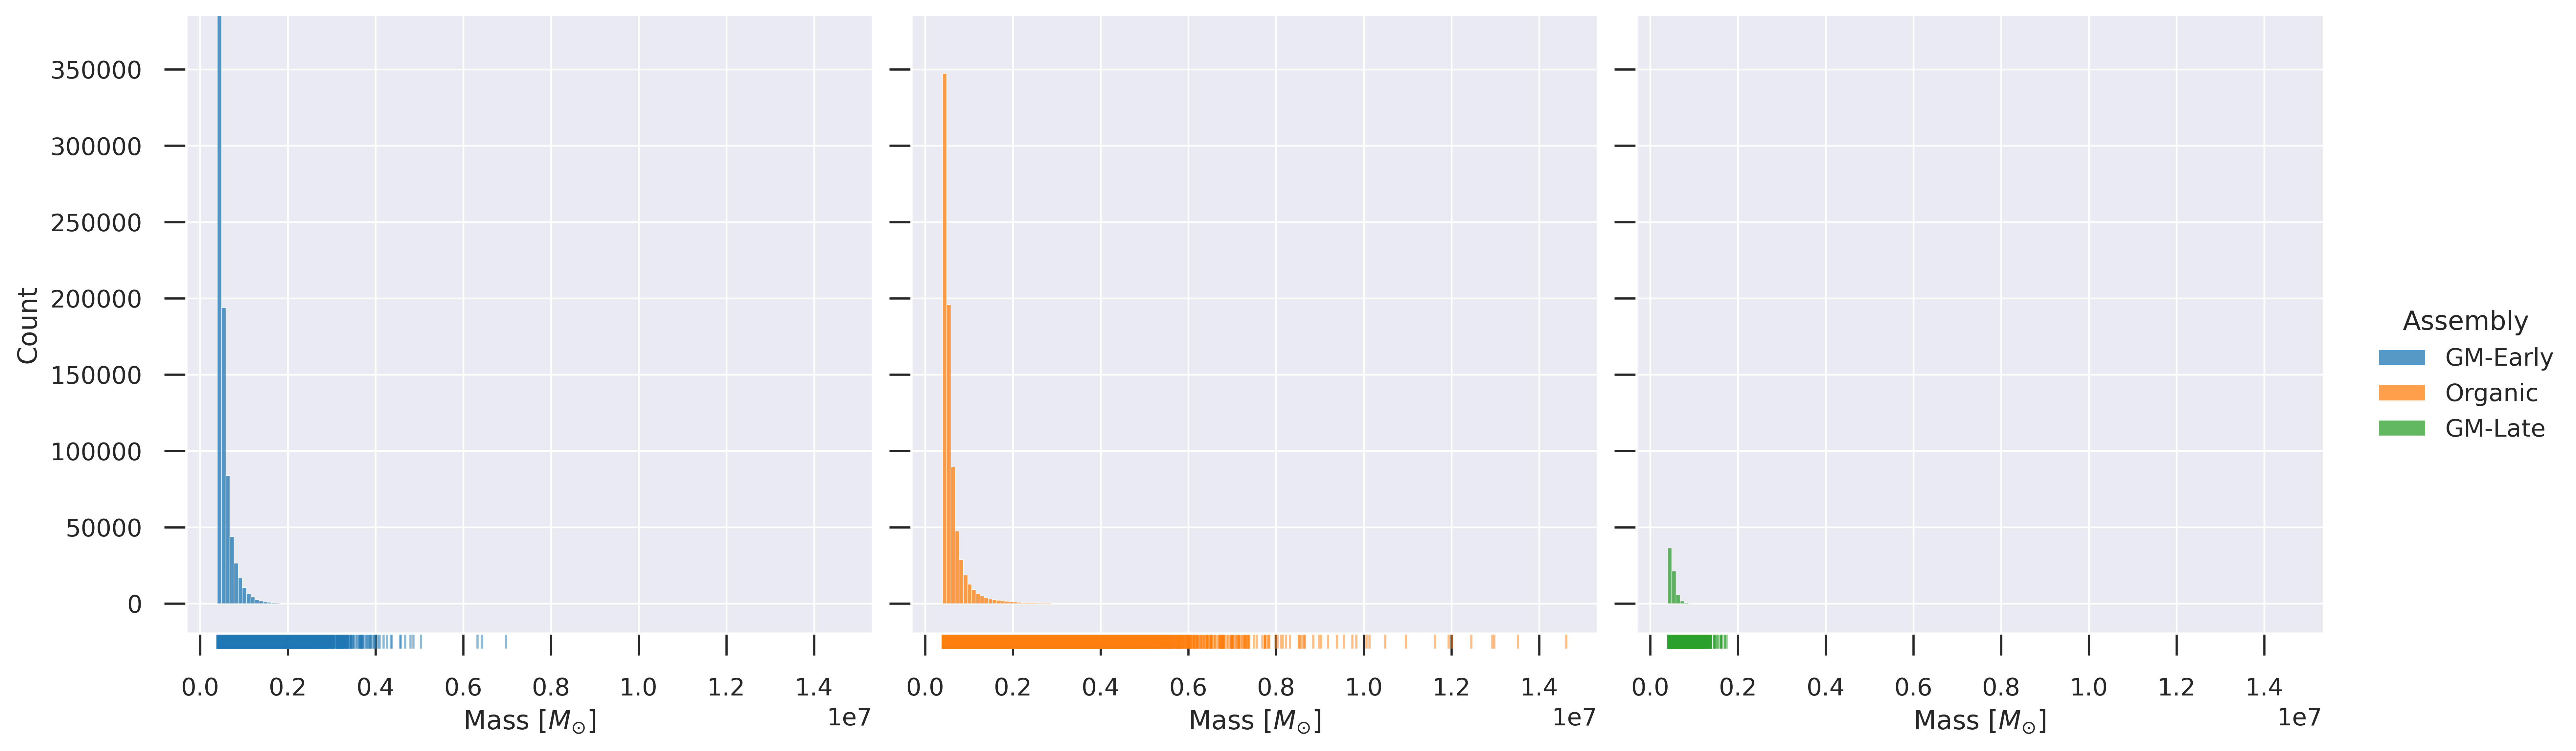
\includegraphics[width=\columnwidth]{../plots/particle_mass_distribution.png}
			\caption{Particles mass distribution combined at all redshifts for three assembly modes. Rugplots on x-axes give an estimate of range of masses involved in the three modes.}
	\end{figure}

	\clearpage

	\begin{figure}
			\centering 
			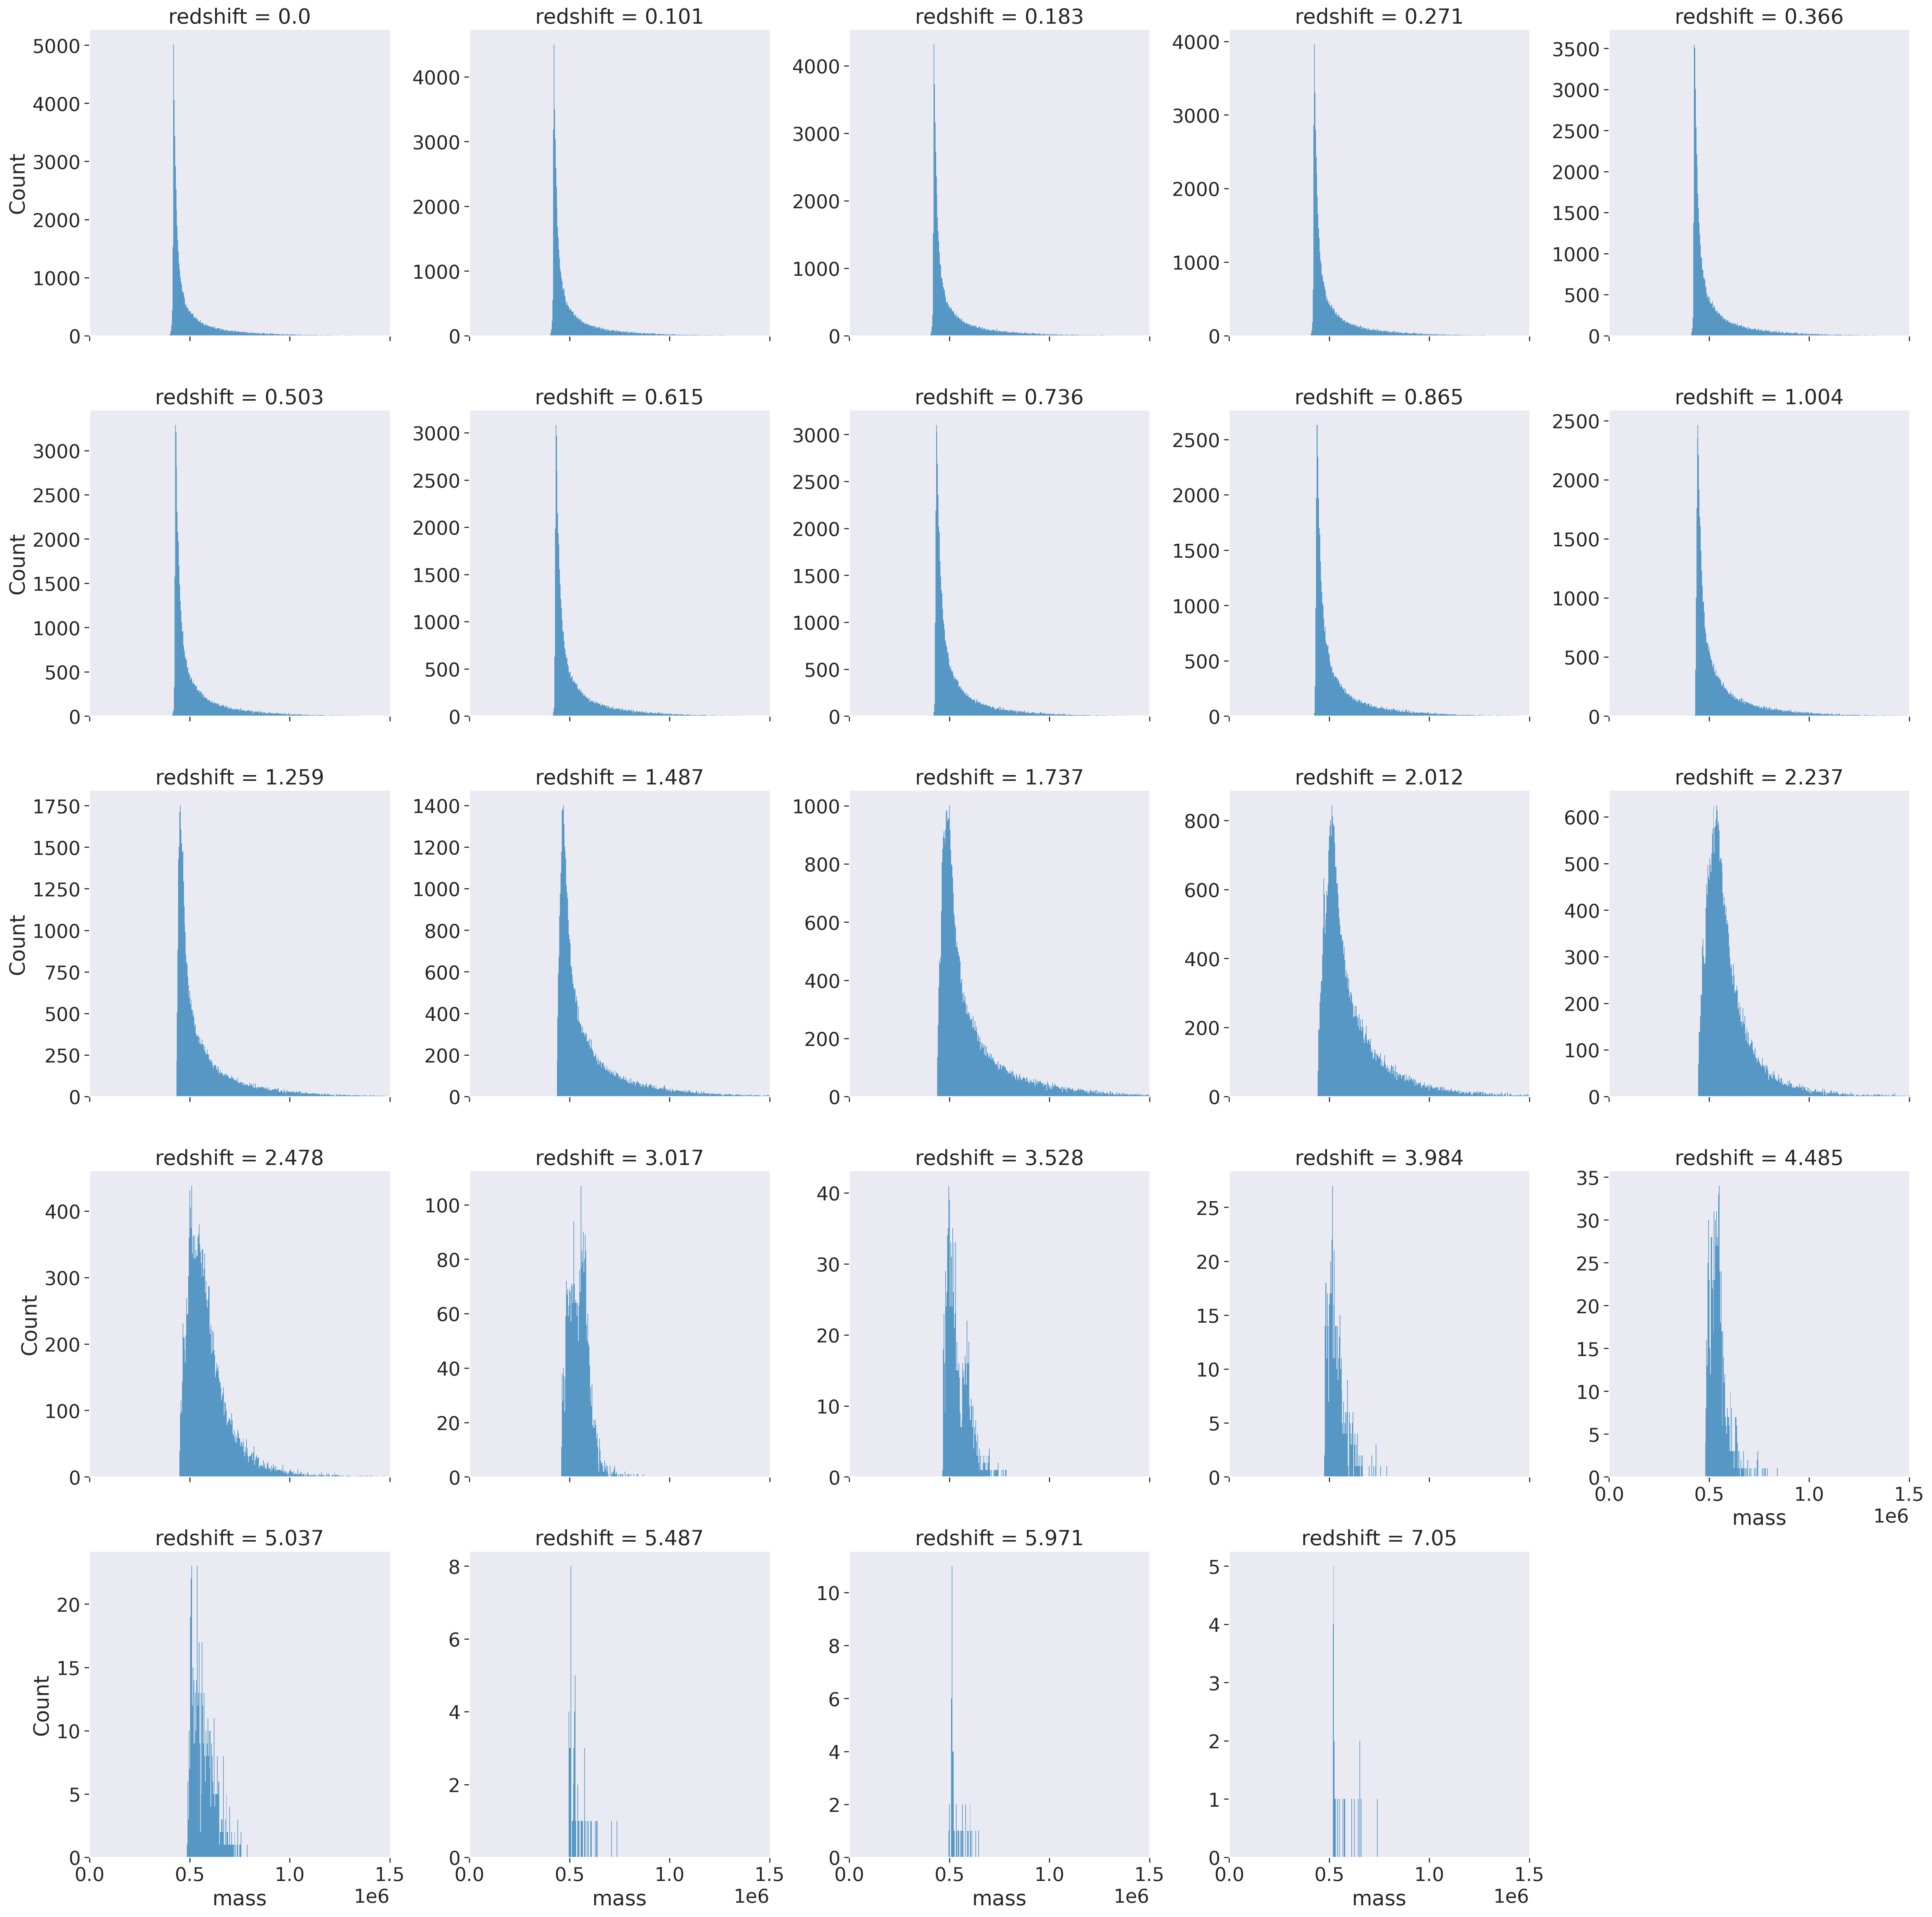
\includegraphics[width=.9\columnwidth]{../plots/mass_distribution_wrt_redshift_GM-Early.png}
			\caption{Particles mass distribution variation with redshift. Note the changing y-axes scales across plots.}
	\end{figure}

\end{document}